% 此文件为编写LaTeX文档的通用模板,包含了一些常用的宏包和设置,可以直接使用或者修改。

\documentclass{article}

% 文档信息设置
\title{ForTesting(Updated)}
\author{Author}
\date{\today}

% 命令支持
\usepackage{xparse}
% 此命令用于支持新的命令定义,其后加入的参数为新命令的名称、参数个数、参数类型、参数默认值、新命令的内容。
% 常见的参数类型有:s(星号)、o(可选参数)、m(普通参数)。

% 行距
\usepackage{setspace}
\linespread{1.4} % 设置行距为1.4倍

% 英文字体支持
\usepackage{fontspec}
\setmainfont[Path="C:/Windows/Fonts/",AutoFakeBold=3,AutoFakeSlant=0.25]{PAPYRUS.TTF} % 设置英文字体,路径为C:/Windows/Fonts,可以根据自己的需要更改。
\setsansfont{Arial}
\setmonofont{Courier New}

% 中文支持
\usepackage{xeCJK}
% \setCJKmainfont[BoldFont=FandolHei,ItalicFont=FandolFang]{FandolSong} % 设置中文字体为宋体
\setCJKmainfont[Path="C:/Windows/Fonts/",AutoFakeSlant=0.225,AutoFakeBold=3]{STKAITI.ttf}
\setCJKsansfont{FandolHei} % 设置中文字体为黑体
\setCJKmonofont{FandolFang} % 设置中文字体为仿宋

% 在文档中临时更换字体:
\newCJKfontfamily{\yh}[AutoFakeSlant=0.225,AutoFakeBold=3]{Microsoft YaHei} % 微软雅黑

\newfontfamily{\fontsh}[AutoFakeSlant=0.225,AutoFakeBold=3,Path="C:/Windows/fonts/"]{FZShouHCGTJW.TTF}
\newCJKfontfamily{\cjksh}[AutoFakeSlant=0.225,AutoFakeBold=3,Path="C:/Windows/fonts/"]{FZShouHCGTJW.TTF}

% 数学符号的支持
\usepackage{amsmath,amssymb,amsthm,amsfonts}
\usepackage{physics}

% 颜色支持
\usepackage{xcolor}

% 表格颜色支持
\usepackage{colortbl}

% 自定义颜色
% 定义自定义颜色的方法有:\definecolor{mycolor}{rgb}{0,0,1},\definecolor{mycolor}{RGB}{0,0,255},\definecolor{mycolor}{HTML}{0000FF}。
% 可选颜色模型有:rgb,RGB,HTML,cmyk,gray,hsb,wave,cmy,hsb,Hsb,tHsb,X11,dvips.

% 画图3D中包含的24种颜色为:内置的white, lightgray, darkgray, black, red, orange, yellow, green, cyan, blue, purple, brown, pink, lime, teal, violet, olive, magenta, maroon, mint, apricot。

\definecolor{backcolor}{rgb}{0.95,0.95,0.92}
\definecolor{codegray}{gray}{0.9}
\definecolor{darkred}{RGB}{139,0,0}

\definecolor{line15}{RGB}{200,179,142} % 上海地铁15号线配色

\definecolor{green1}{RGB}{0, 156, 39} % 深绿
\definecolor{green2}{RGB}{214, 254, 224} % 浅绿

% 文字颜色的命令
\newcommand{\tc}[4][white]{{\fcolorbox{#1}{#2}{\textcolor{#3}{#4}}}} % 此命令接受四个参数,第一个参数为背景颜色,默认为白色,第二个参数为文字背景颜色,第三个参数为文字颜色,第四个参数为文字内容。如:\tc[green]{blue}{lime}{Hello,world!}

% 模拟行内代码的命令
\newcommand{\inl}[1]{{\small{\colorbox{codegray}{\textcolor{darkred}{#1}}}}}

% 可跨页表格
\usepackage{longtable}
\usepackage{booktabs}

% 页边距
\usepackage[margin=1.5cm]{geometry}

% 代码支持
\usepackage{listings}

% 代码样式
\lstset{
    numbers=left,
    numberstyle=\small,
    basicstyle=\ttfamily,
    backgroundcolor=\color{backcolor}, % 背景颜色
    keywordstyle= \color{purple},%设置关键字颜色
    numberstyle= \color{cyan},
    commentstyle= \color{green}, %设置注释颜色
    stringstyle=\color{darkred}, % 字符串颜色
    columns=fullflexible,%可以自动换行
    linewidth=1\linewidth, %设置代码块与行同宽
    showstringspaces=false, %去掉空格时产生的下划的空格标志, 设置为true则出现
    breaklines=true,          % 允许断行
    postbreak=\mbox{$\hookrightarrow$\space},  % 断行时的符号
    keywordstyle=\color{blue},
    commentstyle=\color{green!50!black},
    stringstyle=\color{red},
    showstringspaces=false,
    frame=single
}

% 此命令构建了一个代码块环境,调用时采用如下方式:
% \begin{lstlisting}[language=Cpp]
% your code
% \end{lstlisting}

% 彩色的代码支持:
\usepackage{minted}

% 样式设置
\setminted[cpp]{
    breaklines, frame=single, fontsize=\small, bgcolor=white, linenos
}

% 盒子环境的支持
\usepackage[most]{tcolorbox}
\usepackage{fontawesome5} % 加载 fontawesome5 包,用于添加图标

% 新定义一个简单的盒子环境
\newtcolorbox{blackbox}{
    colback=white,
    colframe=black,
}

% 新定义一个复杂的有标题的盒子环境
\newtcolorbox{testbox}[2][]{
    breakable, % 可分页显示
    enhanced,
    oversize, % 宽距显示
    sharp corners=uphill, % 方角矩形形状
    arc=3mm, % 四角圆的半径
    boxrule=0.4mm, % 盒子边框
    colbacktitle=yellow!20, % 标题背景颜色
    coltitle=black, % 标题颜色
    coltext=yellow!15!black, % 正文颜色
    colback=yellow!40!white, % 正文背景颜色
    colframe=yellow!70!black, % 边框颜色
    fonttitle=\bfseries,
    attach boxed title to top center={yshift=-2mm},
    title={#2},#1
}

\newtcolorbox{textbox}[1][]
{
  title=#1,
  colupper=black, % 设置文本颜色为黑色
  colback=white!95!yellow, % 设置背景颜色为浅黄色
  colframe=black, % 设置边框颜色为黑色
  boxrule=0.7mm, % 设置边框线的粗细
  arc=4mm, % 设置边角的圆润度
  fonttitle=\bfseries\large, % 设置标题字体样式
  left=1em, right=1em, top=0.5em, bottom=0.5em, % 设置内边距
  before upper={\hspace{2mm}\faQuoteLeft~}, % 在内容前添加一个左引号图标
  after upper={~\faQuoteRight} % 在内容后添加一个右引号图标
}


% 行内的盒子环境
\newtcbox{\highl}[1][red]{on line,
 arc=0pt,outer arc=0pt,colback=#1!10!white,colframe=#1!50!black,
 boxsep=0pt,left=1pt,right=1pt,top=2pt,bottom=2pt,
 boxrule=0pt,bottomrule=1pt,toprule=1pt
}

\newtcbox{\chighl}[1][red]{on line,
 arc=7pt,colback=#1!10!white,colframe=#1!50!black,
 before upper={\rule[-3pt]{0pt}{10pt}},boxrule=1pt,
 boxsep=0pt,left=6pt,right=6pt,top=2pt,bottom=2pt
}

% 行内的代码盒子环境的支持:
\NewTotalTCBox{\cmdbox}{ s v }
{verbatim,colupper=white,colback=black!75!white,colframe=white}
{\IfBooleanT{#1}{\textcolor{red}{\ttfamily\bfseries >>> }}
\lstinline[language=command.com,keywordstyle=\color{blue!35!white}\bfseries]^#2^}

% 定义环境:
\newenvironment{sol_box}{
    \begin{tcolorbox}[enhanced, colback=green2, boxrule=0pt, frame hidden,
        borderline west={0.7mm}{0.1mm}{green1},breakable]
}{\end{tcolorbox}}
\newenvironment{sol}[1][]{\begin{sol_box}{\large\textbf{#1}}\newline}{\end{sol_box}}

% 证明环境:
\newenvironment{prf_box}{
    \begin{tcolorbox}[enhanced, colback=lightgray, boxrule=0pt, frame hidden,
        borderline west={0.7mm}{0.1mm}{darkgray},breakable,after upper={$\square$}]
}{\end{tcolorbox}}
\newenvironment{prf}{\begin{prf_box}{\textit{Proof:}\newline}}{\end{prf_box}}


% 图片支持
\usepackage{graphicx}

% 多张图片支持
\usepackage{subcaption}

% 超链接支持
\usepackage{hyperref}

\hypersetup{
    colorlinks=true,
    linkcolor=blue,
    filecolor=magenta,
    urlcolor=cyan
}

% 下脚注
\usepackage[bottom,hang,flushmargin]{footmisc}

% 页眉与页脚的支持
\usepackage{fancyhdr}
\pagestyle{fancy}

% 页眉与页脚的样式设置
\fancyhf{}

\fancyhead[L]{ForTesting}
\fancyhead[R]{页眉(测试)}
\fancyfoot[C]{Page.\thepage}

% 设置页码格式
\renewcommand{\headrulewidth}{0.4pt} % 页眉线宽度
\renewcommand{\footrulewidth}{0.25pt} % 页脚线宽度

% 取消所有的首段缩进的选项:
\setlength{\parindent}{0pt}

% 自定义的非数学运算符:
\newcommand{\armatr}[3]{\mathbb{#1}^{#2\times #3}}

% 自定义的数学运算符
\DeclareMathOperator{\N}{\mathbb{N}}                    % Set of Natural Numbers
\DeclareMathOperator{\Z}{\mathbb{Z}}                    % Set of Integers
\DeclareMathOperator{\Q}{\mathbb{Q}}                    % Set of Rational Numbers
\DeclareMathOperator{\R}{\mathbb{R}}                    % Set of Real Numbers
\DeclareMathOperator{\C}{\mathbb{C}}                    % Set of Complex Numbers

\DeclareMathOperator{\Id}{Id}                           % Identity
\DeclareMathOperator{\FF}{\mathcal{F}}                  % Probability Space
\DeclareMathOperator{\card}{card}                       % Cardinality
\DeclareMathOperator{\Cat}{\mathcal{C}}                 % Category

\DeclareMathOperator{\Hom}{Hom}                         % Set of Homomorphisms
\DeclareMathOperator{\End}{End}                         % Set of Endomorphisms
\DeclareMathOperator{\Aut}{Aut}                         % Set of Automorphisms
\DeclareMathOperator{\Isom}{Isom}                       % Set of Isomorphisms

\DeclareMathOperator{\diag}{diag}                       % Diagonal Matrix

\DeclareMathOperator{\K}{\mathbb{K}}                    % Number Field
\DeclareMathOperator{\F}{\mathbb{F}}                    % Number Field (F)

% Tikz绘图支持
\usepackage{tikz}
\usetikzlibrary{arrows.meta,decorations.pathmorphing,backgrounds,positioning,fit,petri,shapes.misc,graphs,calc,mindmap}

% 自定义tikz命令
\newcommand{\drw}[2]{\draw[->] (#1) -- (#2)}

%---------------------------Pleamble-Ends-Here--------------------------------------------------------------------------------

% 以下文档内容均为测试内容:
\begin{document}

\maketitle

\label{sec:testbegin}
\section{测试文档}

这行文字用于测试普通中文,\textbf{加粗},\textit{斜体}的显示效果。

{\yh 这行文字用于测试临时字体的显示效果。}

{\cjksh 这行文字用于测试临时字体的显示效果。}{\fontsh And English display is also tested.}

This line is used to test the display effect of normal English, \textbf{bold}, and \textit{italic}.

\textsf{This line is used to test the display effect of the font.}

\tc[yellow!80!black]{yellow!20}{yellow!20!black}{这行文字用于测试背景色和文字颜色:}

The \tc[green]{white}{lime}{quick} brown \tc{cyan}{red}{fox} \tc{pink}{darkred}{jumps} over the \tc[black]{blue}{orange}{lazy} \tc{lightgray}{blue}{dog}.

以下内容用于测试数学符号和公式的显示:

$\alpha$、$\beta$、$\gamma$、$\delta$、$\epsilon$、$\zeta$、$\eta$、$\theta$、$\iota$、$\kappa$、$\lambda$、$\mu$、$\nu$、$\xi$、$\pi$、$\rho$、$\sigma$、$\tau$、$\upsilon$、$\phi$、$\chi$、$\psi$、$\omega$、$\Gamma$、$\Delta$、$\Theta$、$\Lambda$、$\Xi$、$\Pi$、$\Sigma$、$\Upsilon$、$\Phi$、$\Psi$、$\Omega$。

$\N$、$\Z$、$\Q$、$\R$、$\C$、$\Id$、$\FF$、$\card$、$\Cat$、$\Hom$、$\End$、$\Aut$、$\Isom$、$\diag$、$\K$、$\F$。

$A\in\armatr{F}{n}{m}.$

Cayley-Hamilton theorem: \[\det(A-\lambda I)=0\]

Central limit theorem: \[\lim_{n\to\infty}\frac{1}{\sqrt{2\pi n}}\int_{-\infty}^{+\infty}e^{-\frac{x^2}{2n}}\dd{x}=1\]

Newton-Leibniz formula: \[\int_a^bf(x)\dd{x}=\eval{F(x)}_{b}^{a}\]

Cauchy Principle Value Examples:\[\PV{\int e^{-x^2}\dd{x}}=\sqrt{\pi}\]

检查矩阵的输入:

$n$阶标准Jordan块具有如下的形式:

\[J_n=\begin{pmatrix}
    \lambda&1& & & \\
    & \lambda&1& & \\
    & &\lambda&\ddots& \\
    & & &\ddots&1\\
    & & & &\lambda
\end{pmatrix}_{n\times n}\]

使用\inl{minted}环境展示的C++代码:

\begin{minted}{cpp}
#include <iostream>
using namespace std;

int main(){
    int n;
    cin>>n;
    for(int i=0;i<n;++i){
        cout<<"Hello, World!"<<endl;
    }
    return 0;
}
\end{minted}

使用\inl{listings}环境展示的C++代码:

\begin{lstlisting}[language=c++]
#include <iostream>
using namespace std;

int main(){
    int n;
    cin>>n;
    for(int i=0;i<n;++i){
        cout<<"Hello, World!"<<endl;
    }
    return 0;
}
\end{lstlisting}

接下来测试盒子环境的显示效果:

\begin{blackbox}
    This is a simple box.
\end{blackbox}

另一种盒子的显示效果:

\begin{testbox}{标题}
    正文
    \tcblower
    分割线下的字段
\end{testbox}

更多的盒子效果:
\begin{textbox}[ForTesting]
    This is a \textbf{tcolorbox}.
\end{textbox}

将用以下环境来盛放各定义,定理,性质与推论:
\begin{sol}[线性代数基本定理]
    \[n=\rank A+\dim\ker \mathcal{A}.\]
\end{sol}

将用以下环境来盛放证明:
\begin{prf}
    不妨假设$m>n$. 矩阵$A^*A$是半正定矩阵,设其秩为$r$,特征值为$\sigma_1^2,\cdots,\sigma_n^2$,设$\alpha_1\cdots,\alpha_n$是由$A^*A$的特征向量组成的规范正交基,$V=(\alpha_1\cdots,\alpha_n)$,则$V$是酉矩阵且\[V^*(A^*A)V=\diag(\sigma_1^2,\cdots,\sigma_n^2)\]
    亦即\[(AV)^*(AV)=\diag(\sigma_1^2,\cdots,\sigma_r^2,0,\cdots,0)\]
    故$AV$的列向量是两两正交的。

    从其中提取这些列向量并归一化得到一组规范正交基$\displaystyle u_1=\frac{AVe_1}{\sigma_1},\cdots, u_r=\frac{AVe_r}{\sigma_r} $;

    任取的左零空间中的一组规范正交基$u_{r+1},\cdots,u_m$,并令\[
    U=(u_1,\cdots,u_r,u_{r+1},\cdots,u_n)
    \]
    则\[AV=(u_1,\cdots,u_r,0,\cdots,0)=(u_1,\cdots,u_r,u_{r+1},\cdots,u_n)\diag(\sigma_1^2,\cdots,\sigma_r^2,0,\cdots,0)=U\Sigma.
    \]
\end{prf}


接下来测试行内盒子的显示效果:

The \highl[green]{quick} brown \highl{fox} \chighl[blue]{jumps} over the \chighl[green]{lazy} \chighl{dog}.

The \cmdbox*{taskkill -pid XXXX} command is used to kill the process with the specified PID.

接下来测试表格的显示效果:

\Large
\begin{longtable}{|c|c|c|}
    \hline
    \rowcolor{blue!20}
    \textbf{姓名} & \textbf{年龄} & \textbf{性别} \\
    \hline
    张三 & \cellcolor{cyan!20} 20 & 男 \\
    \hline
    李四 & 21 & 女 \\
    \hline
    王五 & 22 & 男 \\
    \hline
    赵六 & 23 & 女 \\
    \hline
    \caption{学生信息表}
\end{longtable}
\normalsize

\newpage

接下来测试图片的显示效果:为便于图片显示,我们使用新的一页来呈现。

\begin{figure}[h]
    \centering
    \includegraphics[width=0.5\textwidth]{./fig/test.png}
    \caption{图片1}
    \label{fig:testfig1}
\end{figure}

测试超链接的显示:

该图片可以通过点击\hyperref[fig:testfig1]{\texttt{这里}}查看。

回到文档头:点击\hyperref[sec:testbegin]{\textit{这里}}。

请访问hyperref包的 \href{https://www.ctan.org/pkg/hyperref}{\texttt{官方文档}} 获取更多信息。

\newpage
接下来测试多张图片的显示效果:

\begin{figure}[h]
    \centering
    \begin{subfigure}{0.3\textwidth}
        \centering
        \includegraphics[width=0.9\linewidth]{./fig/test2.png}
        \caption{图片1}
        \label{fig:testfig2}
    \end{subfigure}
    \begin{subfigure}{0.3\textwidth}
        \centering
        \includegraphics[width=0.9\linewidth]{./fig/test3.png}
        \caption{图片2}
        \label{fig:testfig3}
    \end{subfigure}
    \begin{subfigure}{0.3\textwidth}
        \centering
        \includegraphics[width=0.9\linewidth]{./fig/test4.png}
        \caption{图片3}
        \label{fig:testfig4}
    \end{subfigure}
    \caption{使用Stable Diffusion 3.5L生成}
\end{figure}

生成时所用的配置文件在\href{./fig/test.json}{\textbf{这里}}。

检查文章对脚注的支持:

这是一段包含脚注的文字。\footnote{这是第一个脚注,通常用于提供额外的信息。}可以在文中多次使用脚注。\footnote{这是第二个脚注。每个脚注都会自动编号。} 脚注非常有用,特别是在引用资料或提供解释时。

\newpage
测试tikz绘图的显示:

\begin{figure}[h]
    \centering
    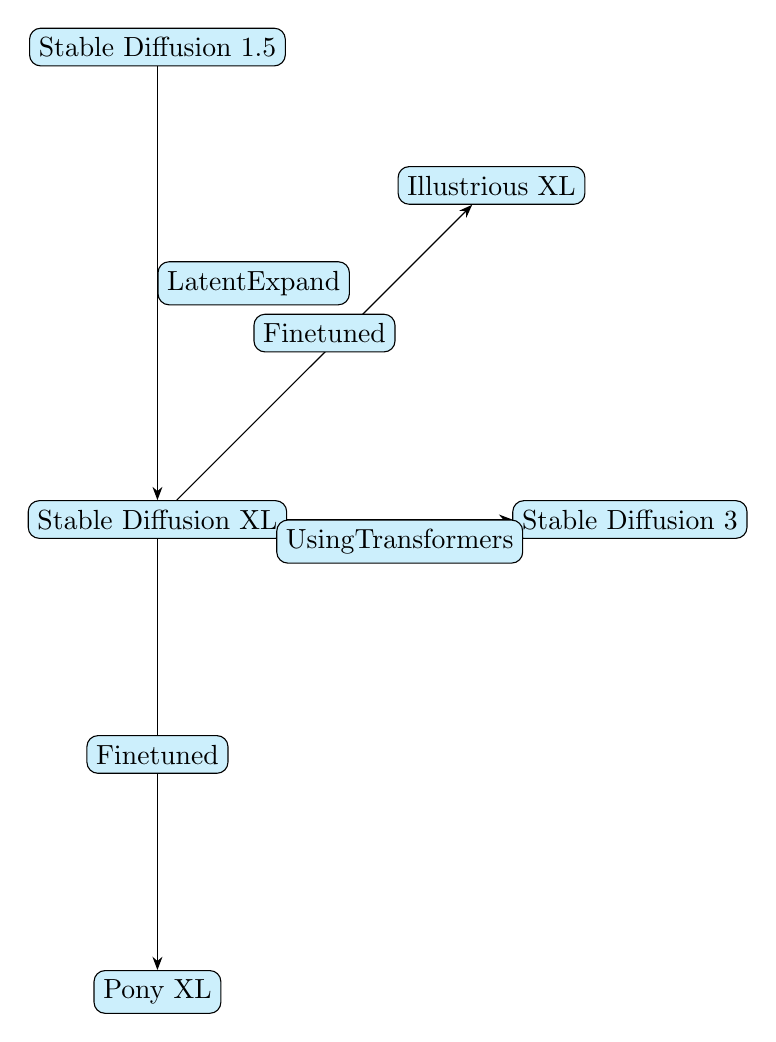
\begin{tikzpicture}[
        node distance=6cm,
        every node/.style={fill=cyan!20,draw,rounded corners},
        >=Stealth % 箭头样式
    ]
        
        % 定义节点
        \node (A) {Stable Diffusion 1.5};
        \node (B) [below of=A] {Stable Diffusion XL};
        \node (C) [right of=B] {Stable Diffusion 3};
        \node (D) [above right of=B] {Illustrious XL};
        \node (E) [below of=B] {Pony XL};
        
        % 连接节点
        \draw [->] (A) -- node[midway,right] {LatentExpand} (B);
        \draw [->] (B) -- node[midway,below] {Using\newline Transformers} (C);
        \draw [->] (B) -- node[midway,above] {Finetuned} (D);
        \draw [->] (B) -- node[midway]{Finetuned}(E);
        
    \end{tikzpicture}
    \caption{Stable Diffusion发展史}
    \label{fig:structure-diagram}
\end{figure}
\newpage
继续测试tikz宏包的绘图功能:
\begin{figure}[h]
  \centering
  \begin{tikzpicture}[
      >=stealth,
      node distance=2.4cm,
      terminal/.style={rectangle,minimum size=6mm,rounded corners=3mm,very thick,draw=black!50,top color=line15!30!white,bottom color=line15,font=\ttfamily}]
      
      % Define nodes
      \node [terminal](A) {祁安路};
      \node [terminal,left of=A] (B) {南大路};
      \node [terminal,left of=B] (BB) {丰翔路};
      \node [terminal,left of=BB] (BC) {锦秋路};
      \node [terminal,left of=BC] (BD) {顾村公园};
      \node [terminal,right of=A] (C) {古浪路};
      \node[terminal,right of=C](CC){武威东路};
      \node[terminal,right of=CC](CD){上海西站};
      \node[terminal,below of=CD](CE){铜川路};
      \node[terminal,left of=CE](E){梅岭北路};
      \node[terminal,left of=E](EA){大渡河路};
      \node[terminal,left of=EA](EB){长风公园};
      \node[terminal,left of=EB](EC){娄山关路};
      \node[terminal,left of=EC](ED){红宝石路};
      \node[terminal,left of=ED](EE){姚虹路};
      \node[terminal,left of=EE](EF){吴中路};
      \node[terminal,below of=EF](CF){桂林路};
      \node[terminal,right of=CF](F){桂林公园};
      \node[terminal,right of=F](FA){上海南站};
      \node[terminal,right of=FA](FB){华东理工大学};
      \node[terminal,right of=FB](FC){罗秀路};
      \node[terminal,right of=FC](FD){朱梅路};
      \node[terminal,right of=FD](FE){景洪路};
      \node[terminal,right of=FE](FF){虹梅南路};
      \node[terminal,below of=FF](CG){景西路};
      \node[terminal,left of=CG](G){曙建路};
      \node[terminal,left of=G](GA){双柏路};
      \node[terminal,left of=GA](GB){元江路};
      \node[terminal,left of=GB](GC){永德路};
      \node[terminal,left of=GC](GD){紫竹高新区};
      \node[terminal,left of=GD](GE){兰香湖南路};
      \node[terminal,left of=GE](GF){汇丰北路};
      \node[terminal,below of=GF](CH){东方美谷大道};
      \node[terminal,right of=CH](H){望园路};
      
      % Draw paths
      \draw[->] (BD) -- (BC);
      \draw[->] (BC) -- (BB);
      \drw{BB}{B};
      \drw{B}{A};
      \drw{A}{C};
      \drw{C}{CC};
      \drw{CC}{CD};
      \drw{CD}{CE};
      \drw{CE}{E};
      \drw{E}{EA};
      \drw{EA}{EB};
      \drw{EB}{EC};
      \drw{EC}{ED};
      \drw{ED}{EE};
      \drw{EE}{EF};
      \drw{EF}{CF};
      \drw{CF}{F};
      \drw{F}{FA};
      \drw{FA}{FB};
      \drw{FB}{FC};
      \drw{FC}{FD};
      \drw{FD}{FE};
      \drw{FE}{FF};
      \drw{FF}{CG};
      \drw{CG}{G};
      \drw{G}{GA};
      \drw{GA}{GB};
      \drw{GB}{GC};
      \drw{GC}{GD};
      \drw{GD}{GE};
      \drw{GE}{GF};
      \drw{GF}{CH};
      \drw{CH}{H};


  \end{tikzpicture}
  \caption{轨道交通15号线运行示意图}
\end{figure}

\newpage

测试其对思维导图能力的支持性:
\begin{figure}[h]
    \centering
    \begin{tikzpicture}[mindmap, concept color=blue!50, text=white, outer sep=0pt,
        every annotation/.style={fill=red!20}]
    \node [concept] (root) {中心主题}
    child[grow=right] {node [concept] {分支1}
        child[concept color=red,grow=30] {node [concept] {子分支1}}
        child[concept color=cyan,grow=0] {node [concept] {子分支2}}
    }
    child {node [concept] {分支2}
        child[grow=330] {node [concept] {子分支3}}
        child[grow=240] {node [concept] {子分支4}}
    };
    \node[extra concept]at(5,-5){其他};
    \node[concept](n2)[circle,minimum size=0.6cm,fill,draw,thick,concept color=green]at(120:4.5){其他}
    child [grow=150,concept color=purple] {
        node [concept] {Conclusions}
    };
    \node [annotation] at (-5,0){The root concept is, in general, the most important concept.};
\end{tikzpicture}
\caption{某种思维导图的形式}
\end{figure}



\end{document}
